
\subsection{Tool-Flow}


\begin{figure*}[t]
\centering
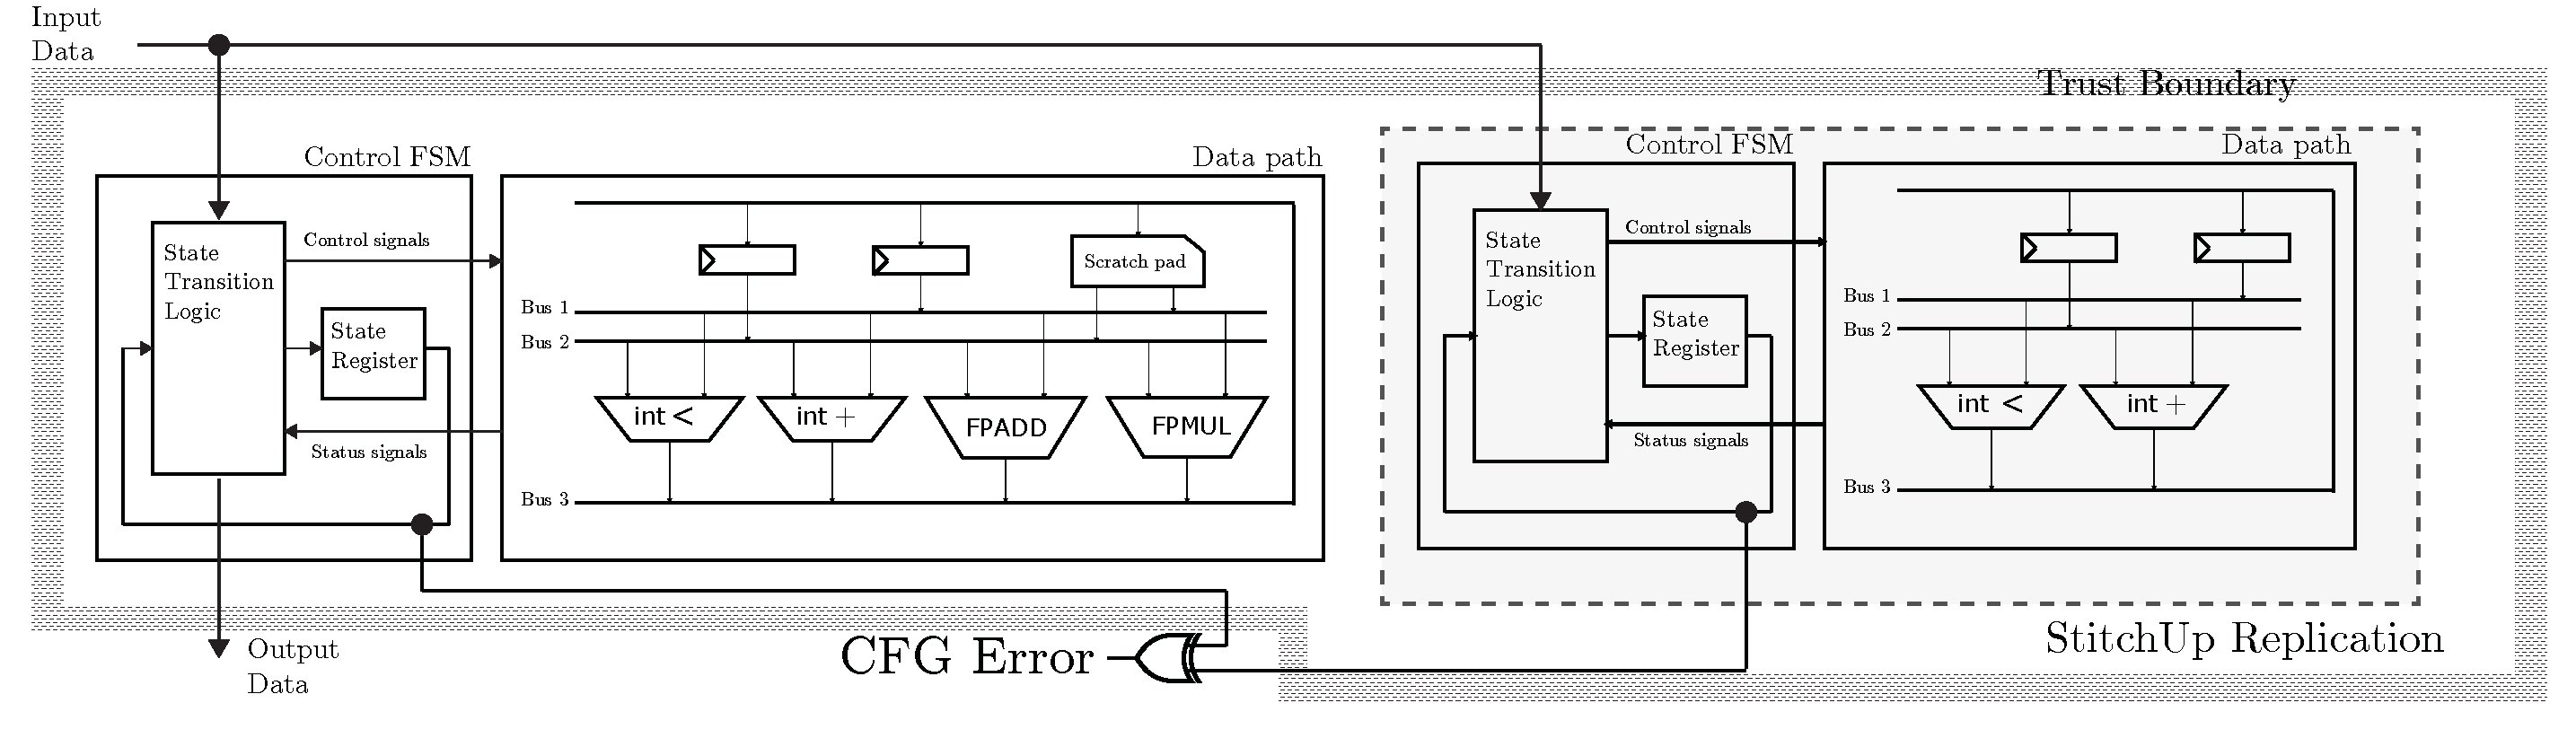
\includegraphics[width=7in]{./imgs/HLSArch.pdf}
\caption{StitchUp Replication for the Matrix Multiplication example, with Trust Boundary}
\label{fig:HLSArch}
\end{figure*}


\begin{figure}[h]
\centering
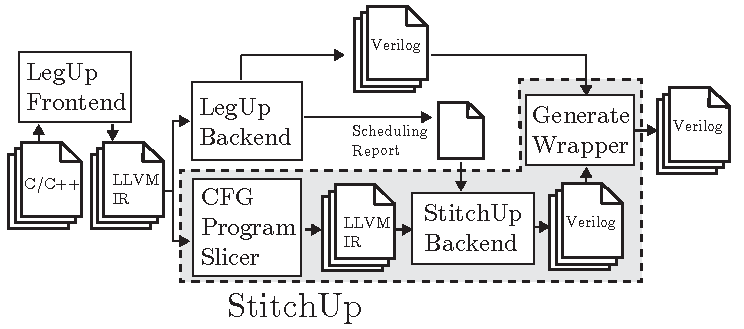
\includegraphics[width=3.5in]{./imgs/tool-flow.pdf}
\caption{Tool Flow Overview diagram}
\label{fig:tool_flow_diagram}
\end{figure}

StitchUp is built as a compile flag for LegUp an open source HLS tool built upon LLVM intermediate representation (LLVM-IR) which has
a similar level of abstraction to assembly code.
LLVM-IR has two important features for writing compiler optimisations:
firstly all instructions are in single static assignment form (SSA) where every variable is only
assigned once; and secondly instructions are grouped into straight-line sequences known as basic blocks (BB)
where there can only one branch in at the start of the block, and one branch out at the end.

Figure \ref{fig:tool_flow_diagram} shows the transformation of an input C program, to a Control-flow protected
Verilog output circuit, with StitchUp specific regions highlighted in grey.
Initially the C input is passed into the LegUp frontend, which is organised as a series of LLVM passes which
to perform various tasks such as annotating instructions with pipelining information.
The LegUp frontend outputs some LLVM-IR which is passed into both the backend of LegUp, to generate the full
original version of the circuit, and the frontend of StitchUp which will generate a control structure only version
of the original circuit.


\begin{figure}[h]
\centering
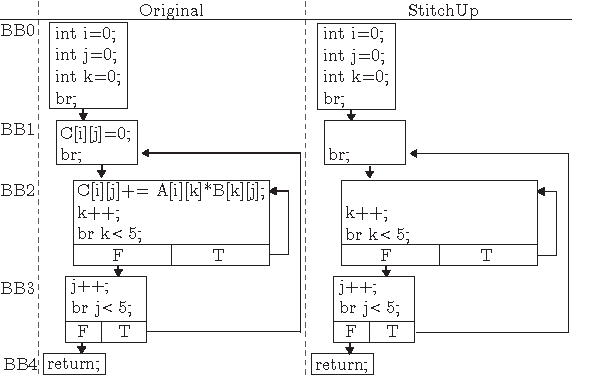
\includegraphics[width=3.5in]{./imgs/mmm_cdfg.pdf}
\caption{Control-Data-Flow Diagram for Matrix Multiplication example}
\label{fig:mmm_cdfg}
\end{figure}

\subsection{Extracting the Control Instruction Set}
The LLVM-IR which is passed into the frontend of StitchUp is naturally arranged into a Control and Dataflow graph (CDFG) format,
where each node of the graph is a basic block and edges are the branches between them.
An example of the CDFG for the matrix multiplication in listing \ref{lst:MMM} is shown on the left in Figure \ref{fig:mmm_cdfg}.

The aim of the StitchUp frontend is to extract all SSA instructions that influence any branch decision and collect them into what
we refer to as a Control Structure Instruction Set (CSIS), which can then be used to generate a control structure only circuit.
In Figure \ref{fig:mmm_cdfg} the original CDFG and StitchUp CDFG can be seen side by side, the CSIS for this example
is every instruction within the StitchUp CDFG and it can be seen that the floating point inner dot product calculation
is not there since it has no impact on any control decision.

In order to automatically extract the $CSIS$ a backwards analysis walks up from the final node of the CDFG to the starting node, analysing
the code as it goes and creating a $CSIS_{i}$ where $i$ is the current node.
The overall $CSIS$ for the input is $CSIS_s$ where $s$ is the starting node of the CDFG.
Constructing the $CSIS_i$ for each node $i$ requires the following three steps:
\begin{enumerate}
    \item For all successor nodes, $j$, of $i$ add every element of $CSIS_j$ to $CSIS_i$.
    \item All branch instructions and operands are added to $CSIS_i$
    \item Any instruction within $i$ that is used as an operand by an element of $CSIS_i$ is added to $CSIS_i$
\end{enumerate}

Following through the example in \ref{fig:mmm_cdfg}:
\begin{itemize}
\item initially start at $BB4$ attempting to build $CSIS_{BB4}$:
since $BB4$ has no successor nodes the first step is skipped, however for the second step the \lstinline{return}
instruction is added to $CSIS_{BB4}$, and the third step is skipped since no other instructions exist.

\item Moving backwards to $BB3$ the first step adds every element of $CSIS_{BB4}$ to $CSIS_{BB3}$ to give 
$CSIS_{BB3}=$ \{\lstinline{return}\}, then since $CSIS_{BB1}$ is currently empty nothing is added from here; the second step then adds the conditional branch and it's operand
instruction to the current set to give $CSIS_{BB3}= $\{\lstinline{return}, \lstinline{br j<5}\} ;
finally for step 3 \lstinline{j} is used in a member of $CSIS_{BB3}$ in \lstinline{br j<5} so the instruction
\lstinline{j++} is added to $CSIS_{BB3}$. This means that at this point $CSIS_{BB3} =$
\{\lstinline{return},\lstinline{br j<5}, \lstinline{j++}\}

\item For $BB2$ in the first step we take all the elements from the successor node $BB3$, and ignore the fact
that it has itself as a successor, so that we get $CSIS_{BB2} =$ \{\lstinline{return},\lstinline{br j<5}, \lstinline{j++}\}.
Then just like before we can add the branch instruction, \lstinline{br k<5}, using rule 2 and the incrementor for the branch
conditional variable \lstinline{k} using rule 3. 
The instruction \lstinline{C[i][j] += A[i][k]*B[k][j]} is not added to $CSIS_{BB2}$ since no instruction
within $CSIS_{BB2}$ depends on it. This leaves 

\end{itemize}

The analysis will continue in this fashion looping over all the Basic Blocks until a fixed
point on every $CSIS$ is obtained.
Once this has been completed it then uses the topmost $CSIS$, in this case $CSIS_{BB0}$ to
generate an LLVM-IR program containing only the control structure of the original
source.

The output of the StitchUp frontend along with the scheduling report from LegUp
implementation of the original circuit are passed into the StitchUp backend, which identical
to the LegUp Backend with a few modifications to the FSM generation.
LegUp schedules operations in such a way that if an instruction requires more than a single
clock cycles to execute then an FSM state is created for each clock cycle.
This means that if instructions are removed via the StitchUp analysis then potentially
the FSM for the StitchUp circuit could be generated missing these extra scheduling states.
For this reason the scheduling report is used to detect instances of where this situation has occurred,
and include these lost states into the StitchUp FSM.


Finally the wrapper scripts take the original LegUp circuit and the StitchUp circuit and
connect them together.
To do this the scripts expose the FSM state registers for each of the circuits and
generate logic to inspect them every clock cycle.
AXI interfaces are also generated, so that the circuits can be easily tested on Xilinx Zynq devices.
